% FINAL camera-ready compact figure preview — ACM sigconf 10pt twocolumn.
% Pair native PDFs at 0.495\columnwidth (scale ≈ 1). No subfigure / no (a)/(b).
\documentclass[sigconf,anonymous,10pt]{acmart}
\usepackage{graphicx}
\setcounter{topnumber}{4}
\renewcommand{\topfraction}{0.92}
\renewcommand{\textfraction}{0.05}
\renewcommand{\floatpagefraction}{0.85}
\setcopyright{none}
\settopmatter{printacmref=false, printccs=false, printfolios=true}
\graphicspath{{_preview_links/}}

\title{MD2G-Cast Compact Figure Preview}
\author{Typography audit}
\renewcommand{\shortauthors}{Preview}

\begin{document}
\maketitle

\section{Evaluation}

We evaluate MD2G under the frozen nested-component contract on development
workloads and a sealed Loot holdout. Same-substrate comparisons use Heuristic,
Clustering, and Rule. Canonical utility is
$U=\mathrm{clip}(0.25 R_o+0.60 R_q-0.15 R_b,0,1)$.
Figures~\ref{fig:ton-u-by-strategy}--\ref{fig:ton-h2-secondary} are independent
floats placed in single-column pairs for layout only.

On MAINDEV, mean matched $\Delta U$ versus the strongest same-substrate baseline
is $+0.016$, with MD2G mean $U\approx0.675$. The sign of the matched gap depends
on load: negative at 20 users and positive at 60 and 100 users. Scaling cells at
$u\in\{10,20,40,60,100\}$ reproduce the same crossover. These facts are supporting
context for the compact figures below; they do not change frozen metrics.

\begin{figure}[t]
\noindent
\begin{minipage}[t]{0.495\columnwidth}
  \centering
  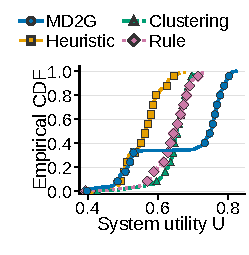
\includegraphics[width=\linewidth]{QoE/QoE_By_Strategy.pdf}
  \caption{Utility ECDF over development workloads.}
  \label{fig:ton-u-by-strategy}
\end{minipage}\hspace{0.01\columnwidth}%
\begin{minipage}[t]{0.495\columnwidth}
  \centering
  
\includegraphics[width=\linewidth]{Buffer/System_Utility_By_Users_scheme1.pdf}
  \caption{Utility versus receiver concurrency.}
  \label{fig:ton-concurrency-crossover}
\end{minipage}
\end{figure}

Fig.~\ref{fig:ton-u-by-strategy} shows the MAINDEV utility distribution.
Fig.~\ref{fig:ton-concurrency-crossover} reports mean $U$ at
$u\in\{10,20,40,60,100\}$. The same-substrate gain appears at medium and high
concurrency; low concurrency remains a limitation. We do not interpret this
crossover as universal dominance, and we do not retune after holdout.

Robustness over content and access is reported next. Each matched block keeps
all launched users in the denominator. Display labels Red\&Black, Longdress, and
Soldier are short names for the same frozen contents. Network rows keep all seven
access profiles, including constrained 4G.

\begin{figure}[t]
\noindent
\begin{minipage}[t]{0.495\columnwidth}
  \centering
  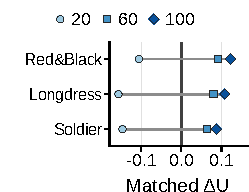
\includegraphics[width=\linewidth]{QoE/QoE_By_Content_DeltaU.pdf}
  \caption{Content-wise matched $\Delta U$ across loads.}
  \label{fig:ton-delta-by-content}
\end{minipage}\hspace{0.01\columnwidth}%
\begin{minipage}[t]{0.495\columnwidth}
  \centering
  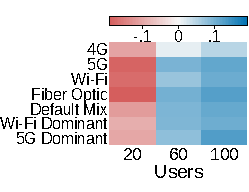
\includegraphics[width=\linewidth]{QoE/QoE_By_Network.pdf}
  \caption{Network-wise matched $\Delta U$ across loads.}
  \label{fig:ton-delta-by-network}
\end{minipage}
\end{figure}

Matched $\Delta U$ in Figs.~\ref{fig:ton-delta-by-content}
and~\ref{fig:ton-delta-by-network} is MD2G minus the strongest same-substrate
baseline. Negative cells at 20 users are retained. The heatmap uses a diverging
scale with no in-cell numerals so the load-conditioned sign change remains the
primary visual message.

Loot remained network-sealed until FINAL DEV freeze and is evaluated as a
315-cell holdout under the same epoch and controller. The holdout pair below
is the load-conditioned story, not an aggregate-only claim.

\begin{figure}[t]
\noindent
\begin{minipage}[t]{0.495\columnwidth}
  \centering
  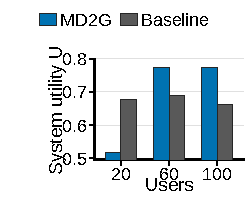
\includegraphics[width=\linewidth]{QoE/Loot_Holdout_DeltaU_By_Users.pdf}
  \caption{Matched utility on unseen Loot.}
  \label{fig:ton-loot-deltau}
\end{minipage}\hspace{0.01\columnwidth}%
\begin{minipage}[t]{0.495\columnwidth}
  \centering
  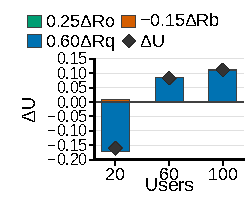
\includegraphics[width=\linewidth]{QoE/Mechanism_Decomposition_Loot.pdf}
  \caption{Matched $\Delta U$ decomposition on Loot.}
  \label{fig:ton-mechanism}
\end{minipage}
\end{figure}

On Loot (Fig.~\ref{fig:ton-loot-deltau}), MD2G trails at 20 users
($\Delta U\approx-0.160$) and leads at 60 and 100 users
($\Delta U\approx+0.083$ and $+0.111$). Fig.~\ref{fig:ton-mechanism} attributes
the signed $\Delta U$ to weighted $R_o$, $R_q$, and $R_b$ terms; it is a
decomposition of the observed utility gap, not an ablation.

The last pair separates architecture from cross-stack systems. Shared MoQ versus
MoQ unicast is not a DASH comparison. GROOT and Rolling remain authentic
DASH/HTTP unicast baselines and are plotted only in Fig.~\ref{fig:ton-h2-secondary}.

\begin{figure}[t]
\noindent
\begin{minipage}[t]{0.495\columnwidth}
  \centering
  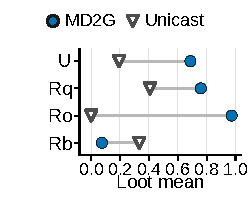
\includegraphics[width=\linewidth]{QoE/MoQ_Shared_vs_Unicast.pdf}
  \caption{Shared MoQ versus MoQ-Unicast on Loot.}
  \label{fig:ton-shared-vs-unicast}
\end{minipage}\hspace{0.01\columnwidth}%
\begin{minipage}[t]{0.495\columnwidth}
  \centering
  
\includegraphics[width=\linewidth]{UX/H2_Cross_Stack_DASH.pdf}
  \caption{Cross-stack utility at 20 and 60 users.}
  \label{fig:ton-h2-secondary}
\end{minipage}
\end{figure}

Fig.~\ref{fig:ton-shared-vs-unicast} isolates delivery architecture (shared MoQ
versus MoQ unicast, $R_o{=}0$), not a controller ranking.
Fig.~\ref{fig:ton-h2-secondary} is a separate cross-stack DASH/HTTP comparison
and must not be read as MoQ unicast.

\end{document}
